\documentclass[english]{article}
\usepackage[T1]{fontenc}
\usepackage[latin9]{inputenc}
\usepackage{geometry}
\geometry{verbose,tmargin=2cm,bmargin=2cm,lmargin=2cm,rmargin=2cm}
\usepackage{float}
\usepackage{textcomp}
\usepackage{amsmath}
\usepackage{amssymb}
\usepackage{graphicx}
\usepackage{setspace}
\usepackage[authoryear]{natbib}
\doublespacing

\makeatletter

%%%%%%%%%%%%%%%%%%%%%%%%%%%%%% LyX specific LaTeX commands.
%% Because html converters don't know tabularnewline
\providecommand{\tabularnewline}{\\}

%%%%%%%%%%%%%%%%%%%%%%%%%%%%%% Textclass specific LaTeX commands.
\newcommand{\lyxaddress}[1]{
	\par {\raggedright #1
	\vspace{1.4em}
	\noindent\par}
}

%%%%%%%%%%%%%%%%%%%%%%%%%%%%%% User specified LaTeX commands.
\usepackage{ae,lmodern}
\usepackage{graphicx}
\usepackage{lineno}
\usepackage{authblk}
\date{}


\renewenvironment{abstract}
 {\small
  \begin{center}
  \bfseries \abstractname\vspace{-.5em}\vspace{0pt}
  \end{center}
  \list{}{
    \setlength{\leftmargin}{.5cm}%
    \setlength{\rightmargin}{\leftmargin}%
  }%
  \item\relax}
 {\endlist}

\DeclareMathOperator\erf{erf}

\makeatother

\usepackage{babel}
\begin{document}
\title{Local intraspecific aggregation in phytoplankton model communities:
spatial scales of occurrence and implications for coexistence}
\author{Coralie Picoche\textonesuperior , William R. Young\texttwosuperior ,
Fr\'e{}d\'e{}ric Barraquand\textonesuperior{}}
\maketitle

\lyxaddress{\noindent \begin{center}
\textonesuperior Institute of Mathematics of Bordeaux, University
of Bordeaux and CNRS, Talence, France\\
\texttwosuperior Scripps Institution of Oceanography, La Jolla, California,
USA
\par\end{center}}

\vspace{-1cm}
\begin{abstract}
The coexistence of multiple phytoplankton species despite their reliance
on similar resources is often explained with mean-field models assuming
mixed populations. In reality, observations of phytoplankton indicate
spatial aggregation at all scales, including at the scale of a few
individuals. Local spatial aggregation can hinder competitive exclusion
since individuals then interact mostly with other individuals of their
own species, rather than competitors from different species. To evaluate
how microscale spatial aggregation could explain phytoplankton diversity
maintenance, an individual-based, multispecific representation of
cells in a realistic hydrodynamic environment is required. We therefore
used as a starting point a mathematically tractable individual-based
model of phytoplankton population dynamics in a viscous and turbulent
environment, and generalize it here to multiple species and three
dimensions. The model is studied through both simulations and the
derivation of spatial moment equations, in connection with point process
theory. The spatial moment equations show a good match between theory
and simulations. We parameterized the model based on phytoplankters\textquoteright{}
ecological and physical characteristics, for both large and small
phytoplankton. Defining a zone of potential interaction as the overlap
between nutrient depletion volumes, we show that local species composition---within
the range of possible interactions---depends on the size class of
phytoplankton. In large phytoplankton, individuals are surrounded
by cells from other species, while in small phytoplankton, individuals
remain in mostly monospecific clusters. Spatial structure therefore
favours intra- over inter-specific interactions for small phytoplankton,
which likely contributes to coexistence mechanisms, while other factors
behind diversity maintenance must be examined for large phytoplankton.
\end{abstract}
\textbf{Keywords}: aggregation; coexistence; individual-based model;
phytoplankton; spatial moment equations; spatial point process 

$^{*}$corresponding author: \verb|coralie.picoche@u-bordeaux.fr|

%\linenumbers
\doublespacing

\clearpage{}


\section*{Introduction}

Phytoplankton communities are among the most important photosynthetic
groups on Earth, being at the bottom of the marine food chain, and
responsible for approximately half the global primary production \citep{field_primary_1998}.
Their contribution to ecosystem functions is only matched by their
contribution to biodiversity. Indeed, phytoplankton communities are
characterized by a surprisingly high biodiversity. For example, a
single sample as small as a few mL can contain up to seventy species
\citep{REPHY_db,widdicombe_2021}. This observation has led to the
formulation of the so-called ``paradox of the plankton'' \citep{hutchinson_paradox_1961},
which refers to the conflict between the observed diversity of species
competing for similar resources in a seemingly homogeneous environment,
and theoretical expectations of a few species outcompeting the others.
Phytoplankton models for coexistence are now almost as diverse as
their model organisms \citep{record_paradox_2014} and some benefit
from the support of coexistence theory, which proposes mechanisms
to escape from competitive exclusion \citep{li_effects_2016,chesson_updates_2018}.
However, most of these models consider mean-field dynamics at the
microscale. Such assumption needs to be challenged, as field observations
themselves have revealed phytoplankton patchiness for more than a
century \citep{bainbridge_size_1957,stocker_marine_2012}, from the
macro- to the micro-scale \citep{leonard_interannual_2001,doubell_high-resolution_2006,font-munoz_advection_2017}.

Phytoplankton patchiness can at least be partly explained by the hydrodynamics
of their environment: the size of these organisms being mostly below
the size of the smallest eddy (i.e., the Kolmogorov scale) in a typical
environment such as the ocean, phytoplankton individuals are embedded
in viscous micro-structures \citep{peters_effects_2000} while phytoplankton
populations are being displaced by a turbulent flow at slighly larger
scales \citep{martin_phytoplankton_2003,prairie_biophysical_2012}.
Phytoplankton organisms therefore live in an environment where fluid
viscosity dominates at the scale of an individual but effects of turbulence
can be seen as soon as one considers the volume required for a small
population of those individuals \citep{estrada_effects_1987,prairie_biophysical_2012}
. 

This leads us to consider demography in the context of this environmental
variation created by hydrodynamics processes. Individual-based models
provide a convenient depiction of population dynamics and movement
at the microscale \citep{hellweger_bunch_2009}. In this framework,
population growth is a result of individual births and deaths. Aggregation
of particles can emerge from local reproduction coupled with limited
dispersal, which can happen in a fluid where turbulence and diffusion
are not too high too disperse kin aggregates \citep{young_reproductive_2001}.
Such aggregation can affect the dynamics of the populations at the
community level: even when interactions are identical between individuals
of the same species (conspecifics) or between individuals of different
species (heterospecifics), the combination of local reproduction and
same-scale high dispersal limitation and strong interactions leads
to stronger intraspecific interactions than interspecific interactions
at the population level, a major stabilizing mechanism \citep{detto_stabilization_2016}.
Basically, a high intra-to-interspecific interaction strength ratio
makes a species control its abundance more than it controls the abundance
of other species, which is associated with coexistence in theoretical
models \citep{levine_importance_2009,barabas_self-regulation_2017}
and often observed in the field at the population level \citep{adler_competition_2018,picoche_strong_2020}.
Therefore, the microscale spatial distribution of individuals likely
affect the interaction structure within a community, and may sustain
diversity.

Some models of phytoplankton populations already exist at the microscale,
i.e. near the Kolmogorov scale, between 1 mm and 1 cm in an oceanic
environment \citep{barton_impact_2014}. Most of these models focus
on a single species and the clustering of its individuals \citep{young_reproductive_2001,birch_bounding_2007,bouderbala_3d_2018,breier_emergence_2018}.
They share a similarity to dynamic point process models \citep{law_population_2003,bolker_spatial_1999,plank_spatial_2015}
developed initially with larger organisms in mind. When phytoplankton
individual-based models consider multiple types of organisms, they
focus for now on how organisms with opposite characteristics \citep[e.g., increase vs decrease in density with turbulence in][]{borgnino_turbulence_2019,arrieta_fate_2020}
segregate spatially, or on coexistence for species that have constrasted
trait values \citep[e.g., size in][]{benczik_coexistence_2006}. This
is quite useful to understand how species with marked differences
coexist. However, the difficulty of the coexistence problem is precisely
that we have to explain how closely related species or genera (e.g.,
within diatoms), many of whom have similar size, buoyancy, chemical
composition, etc., manage to coexist within a single trophic level.
This requires to model \emph{similar} species in spatially realistic
environment and measure whether they aggregate or segregate in space.

To do so, we build a multispecific version of the Brownian Bug Model
(BBM) of \citet{young_reproductive_2001}, an individual-based model
which includes a chaotic advection process mimicking a turbulent fluid
flow, passive diffusion of organisms, as well as stochastic birth
and death processes. The initial version of this model \citep{young_reproductive_2001}
coupled limited dispersal and local reproduction with ocean-like microscale
hydrodynamics, and showed spatial clusters of individuals of the same
species. It was limited to a single species and a two-dimensional
environment. Furthermore, the model was not strongly quantitative
\citep{picoche_rescience_2022} in the sense that parameters were
not informed by current knowledge on phytoplankton biology (numbers
of cells per liter, diffusion characteristics, etc.). As phytoplankton
organisms live in a three-dimensional environment, informing the model
with realistic parameters required us to shift to three dimensions.
We also extend the model to multiple species, and consider two size
classes for our phytoplankton communities, which are either made of
nanophytoplankton (3 \textmu m diameter, $\approx10^{6}$ C/L) or
microphytoplankton (50 \textmu m, $\approx10^{4}$ C/L). We populate
each community with 3 to 10 different species.

The Brownian Bug model (in its original single-species form as in
the multispecies version considered here) is linked to spatial branching
processes. Without advection, it combines a continuous-time, discrete-state
model for population growth and a continuous-time, continuous-space
Brownian motion for particle diffusion \citep{birch_master_2006}.
It is further complexified by the presence of a turbulent fluid flow
in \citet{young_reproductive_2001,picoche_rescience_2022} as well
as here. In spite of this complexity, it remains possible to derive
the dynamics of pair density functions, which quantify the degree
of intra- and interspecific clustering of organisms, via correlations
between positions of organisms (see Methods). This means that in addition
to simulations, we can keep track analytically of spatial structure.
Furthermore, because we do not consider direct interactions between
organisms, the multispecies spatial point process that represents
the stable state of the Brownian Bug model is mathematically a random
superposition of spatial point processes for each species \citep{illian2008statistical}.
This enables us to derive, in addition to pair correlation functions,
analytical formulas for the species composition of the neighbourhood
of an individual, which are more readily ecologically interpreted
than pair density or correlation functions. 


\section*{Models and spatial statistics}

\subsection*{Brownian bug model}

The Brownian Bug Model (BBM) describes the dynamics of particles going
through demographic processes in a turbulent and viscous environment,
in continuous space and time. It has been developed in its two-dimension,
monospecific version in \citet{young_reproductive_2001}, which we
now extend to three dimensions and to $S$ species.

In this model, we consider a community of particles, each individual
being characterized by its species $i$ and its position $\mathbf{x}^{T}=(x,\,y,\,z)$.
Within a given community, all species are equivalent and share the
same parameters. The population dynamics are modeled by a linear birth-death
process with birth rate $\lambda$ and death rate $\mu$. Each particle
independently follows a Brownian motion with diffusivity $D$, and
is advected by a common stochastic flow modeling the turbulence with
stretching parameter $\gamma$, meaning that the separation $s(t)$
between two points previously on top of each other follows $s(t)\varpropto e^{3\gamma t}$.
We focus here on ecologically relevant quantities which can be extracted
from this model, both analytically and numerically. 

For numerical simulations, this model needs to be discretized. During
each time step of duration $\tau$, events unroll as follow:
\begin{enumerate}
\item demography: each particle can either reproduce with probability $p=\lambda\tau$
(forming a new particle of the same species $i$ at the same position
$\mathbf{x}$), die with probability $q=\mu\tau$, or remain unchanged
with probability $1-p-q$.
\item diffusion: each particle moves to a new position $\mathbf{x}(t+t')=\mathbf{x}(t)+\delta\mathbf{x}(t)$
where each element of $\delta\mathbf{x}(t)$ follows a Gaussian distribution
$\mathcal{N}(0,\Delta)$ with $D=\frac{\Delta^{2}}{2\tau}$ the diffusivity. 
\item turbulence: each particle is displaced by a turbulent flow, following
the Pierrehumbert map \citep{pierrehumbert_tracer_1994}, adapted
in its three-dimension version \citep{ngan_scalar_2011}. The shift
from continuous to discrete time is described in Section S1 in the
Supplementary Information.
\end{enumerate}
\[
\begin{cases}
x(t+\tau) & =x(t+t')+U\tau/3\cos\left(ky(t+t')+\phi(t)\right)\\
y(t+\tau) & =y(t+t')+U\tau/3\cos\left(kz(t+t')+\theta(t)\right)\\
z(t+\tau) & =z(t+t')+U\tau/3\cos\left(kx(t+\tau)+\psi(t)\right)
\end{cases}
\]

where $U$ is the maximum velocity of the particle, $k=2\pi/L_{s}$
is the wavenumber for the flow at the length scale $L_{s}$ (see below)
and $\phi(t)$, $\theta(t)$, $\psi(t)$ are random phases uniformly
distributed between $0$ and $2\pi$. Particles are distributed in
a cube of side $L$, with periodic boundary conditions.

\subsection*{Characterization of the spatial distribution}

Let $W$ be the observation window (in our case, the whole cube, which
we never subsample hereafter). The state of the system at time $t$
can be described as a collection of $S$ populations, where the population
of species $i$ is made of $n_{i}$ particles randomly distributed
in $W$, with positions $\boldsymbol{X}_{i}(t)=[\boldsymbol{x}_{1,i}(t),\boldsymbol{x}_{2,i}(t),...\boldsymbol{x}_{n_{i},i}(t)]$.
$\boldsymbol{X}(t)=[\boldsymbol{X}_{1}(t),\ldots,\boldsymbol{X}_{S}(t)]$
arises from a stochastic and spatial individual-based model changing
through time, but can also be analyzed as a spatial point process
at time $t$. We note that the point distributions remain the same
for all translations $\xi$ (i.e., the point process described by
the set $\boldsymbol{X}=[\boldsymbol{x}_{1},\boldsymbol{x}_{2},...\boldsymbol{x}_{k}]$
is the same as $\boldsymbol{X_{\xi}}=[\boldsymbol{x}_{1}+\xi,\boldsymbol{x}_{2}+\xi,...\boldsymbol{x}_{k}+\xi])$:
the process is stationary.

One of the most common methods to describe a spatial point process
is through its spatial moments, that can be theoretically derived
and allow us to check our simulations. However, the spatial moments
of a process are merely statistical indicators which then need to
be related to more easily ecologically interpretable quantities. This
is the role of the dominance index, which we present below.

\subsubsection*{Spatial moments}

The first-order moment is the intensity of the process, or mean concentration
of particles $C_{i}=\frac{N_{i}(W)}{V(W)}$ where $N_{i}(W)$ is the
number of particles of species $i$ in the cube $W$ and $V(W)=L^{3}$
is the volume of the cube; it does not give any information regarding
the spatial distribution of particles, and possibly their spatial
correlations.

The second-order product density, or pair density $G(r,t)$, is the
expected density of pairs of points separated by a distance $r$ \citep{law_population_2003}.
A similar characteristic can be used for marked spatial point process.
In our case, the marks are the species, and we can define $G_{ij}(r,t)$,
so that $G_{ij}(r,t)d\mathbf{x}_{A}d\mathbf{x}_{B}$ is the probability
of finding an individual of species $i$ in volume $d\mathbf{x}_{A}$
and an invidual of species $j$ in volume $d\mathbf{x}_{B}$, and
the distance between the centers of $d\mathbf{x}_{A}$ and $d\mathbf{x}_{B}$
is equal to $r$ (pages 219 and 325 in \citealp{illian2008statistical}).
We show in \citet{picoche_rescience_2022} that the intraspecific
pair density $G_{ii}(r,t)$, in three dimensions, is a solution of
eq. \ref{eq:Young3D}:

\begin{equation}
\frac{\partial G_{ii}}{\partial t}(r,t)=\frac{2D}{r^{2}}\frac{\partial}{\partial r}\left(r^{2}\frac{\partial G_{ii}}{\partial r}\right)+\frac{\gamma}{r^{2}}\frac{\partial}{\partial r}\left(r^{4}\frac{\partial G_{ii}}{\partial r}\right)+2(\lambda-\mu)G_{ii}+2\lambda C_{i}\delta(\boldsymbol{r}).\label{eq:Young3D}
\end{equation}

The pair correlation function $g_{ij}(r,t)$, or pcf, can be derived
from the pair density (eq. \ref{eq:def_pcf}). It is equal to one
when the spatial distribution of species $i$ individuals is random
relative to species $j$ individuals.

\begin{equation}
g_{ij}(r,t)=\frac{G_{ij}(r,t)}{C_{i}C_{j}}\label{eq:def_pcf}
\end{equation}

By integration of eq. \ref{eq:Young3D}, with $\lambda=\mu$ (population
at equilibrium), the intraspecific pcf $g_{ii}(r,t)$ follows eq.
\ref{eq:pcf_intraspecific} (see eqs. \ref{eq:steady_state} to \ref{eq:pcf_noadv_bbm}
in the Appendices for a derivation). The system stabilizes in the
presence of advection ($U>0$), but depends on time in its absence.
\begin{equation}
g_{ii}(r,t)=\begin{cases}
1+\frac{\lambda}{4D\pi rC_{i}}\left\{ 1-\erf\left(\frac{r}{\sqrt{8Dt}}\right)\right\}  & \text{for }U=0\\
1+\frac{\lambda}{2\pi C_{i}}\left(\frac{\sqrt{\gamma}\arctan\left(\frac{\sqrt{\gamma}r}{\sqrt{2D}}\right)}{2^{3/2}D^{3/2}}+\frac{1}{2Dr}-\frac{\pi\sqrt{\gamma}}{2^{5/2}D^{3/2}}\right) & \forall U>0
\end{cases}\label{eq:pcf_intraspecific}
\end{equation}

As populations of different species do not directly interact, each
population is an independent realization of a point process, which
means that the distribution of all particles within the community
constitutes a random superposition of stationary point processes and
$g_{ij}(r,t)=1\text{ }\forall i\neq j,\,\forall U$ \citep[ p. 326, eq. 5.3.13]{illian2008statistical}.\medskip{}

Related to the pair correlation function is Ripley's $K$-function
$K(r)$. Its marked version, $K_{ij}(r)$, is the average number of
points of species $j$ surrounding a particle of species $i$ within
a sphere of radius $r$ \citep{illian2008statistical}.

\begin{equation}
\forall r\geq0\textmd{, }K_{ij}(r)=\frac{1}{C_{j}}\mathbb{E}_{i}\left(N_{j}\left(b(o,r)\right)\right)
\end{equation}

where $\mathbb{E}_{i}$ is the expectation with respect to points
of species $i$ and $N_{j}\left(b(o,r)\backslash\{o\}\right)$ is
the number of points of species $j$ in the sphere of radius $r$
centred on $o$, not counting $o$ itself. The relationship between
$K_{ij}(r)$ and $g_{ij}(r)$ is given in eq. \ref{eq:pcf_to_K}.

\begin{equation}
g_{ij}(r)=\frac{K_{ij}'(r)}{4\pi r^{2}}\label{eq:pcf_to_K}
\end{equation}

Combining eq. \ref{eq:pcf_intraspecific} and eq. \ref{eq:pcf_to_K}
(derivation in eqs. \ref{eq:start-K} to \ref{eq:end_K} in the Appendices),
we can show that:

\begin{doublespace}
\begin{equation}
K_{ii}(r,t)=\begin{cases}
\frac{4}{3}\pi r^{3}+\frac{\lambda}{C_{i}D}\left(\frac{r^{2}}{2}-\frac{1}{2}\erf(\frac{r}{\sqrt{8Dt}})(r^{2}-4Dt)-\frac{\sqrt{2Dt}r}{\sqrt{\pi}}e^{-r^{2}/8Dt}\right) & \text{for }U=0\\
\frac{4}{3}\pi r^{3}+\frac{2\lambda}{C_{i}}\left(\frac{r^{2}}{6D}+\frac{\sqrt{\gamma}r^{3}\arctan(\sqrt{\frac{\gamma}{2D}}r)}{6\sqrt{2}D^{3/2}}+\frac{\log\left(\gamma\frac{r^{2}}{2D}+1\right)}{6\gamma}-\frac{\sqrt{\gamma}\pi r^{3}}{12\sqrt{2}D\sqrt{D}}\right) & \forall U>0
\end{cases}\label{eq:K_intraspecific}
\end{equation}

\end{doublespace}

For random superposition of stationary point processes, $K_{ij}(r,t)=\frac{4}{3}\pi r^{3}$
whenever $i\neq j$ \citep[p. 324, eq. 5.3.5]{illian2008statistical}.

\subsubsection*{Dominance index}

The dominance index \citep[defined in Table S1 in the Supporting Information of][]{wiegand_how_2007}
is the ratio between the number of conspecifics and the number of
individuals of all species surrounding a given individual.

 Let $M_{i.}(r)$ be the average number of individuals within a circle
of radius $r$ around an individual of species $i$, which can also
be written with Ripley's $K$-function as $M_{i.}(r)=C_{.}K_{i}(r)$.
$M_{ii}(r)$ corresponds to the conspecific neighbourhood and $M_{io}(r)$
corresponds to individuals of all other species. We can then define
$D_{i}$ with eq. \ref{eq:dominance}.

\begin{doublespace}
\begin{equation}
\begin{array}{ccc}
D_{i}(r) & = & \frac{M_{ii}(r)}{M_{ii}(r)+M_{io}(r)}\\
 & = & \frac{C_{i}K_{ii}(r)}{\sum_{j=1}^{S}C_{j}K_{ij}(r)}
\end{array}\label{eq:dominance}
\end{equation}

\end{doublespace}

When individuals of the same species $i$ tend to cluster, $D_{i}(r)$
tends to 1 while it tends to the proportion of individuals of species
$i$ in the whole community when the distribution is uniform (see
examples in Section S2 of the SI).

Using eq. \ref{eq:K_intraspecific} and \ref{eq:dominance}, we obtain
a theoretical formula for the dominance index (see corresponding figure
in Section S3 of the SI):

\begin{doublespace}
\begin{equation}
D_{i}(r,t)=\begin{cases}
\frac{C_{i}\left[\frac{4}{3}\pi r^{3}+\frac{\lambda}{C_{i}D}\left(\frac{r^{2}}{2}-\frac{1}{2}\erf(\frac{r}{\sqrt{8Dt}})(r^{2}-4Dt)-\frac{\sqrt{2Dt}r}{\sqrt{\pi}}e^{-r^{2}/8Dt}\right)\right]}{\sum_{j_{=1}}^{S}C_{j}\frac{4}{3}\pi r^{3}+\frac{\lambda}{D}\left(\frac{r^{2}}{2}-\frac{1}{2}\erf(\frac{r}{\sqrt{8Dt}})(r^{2}-4Dt)-\frac{\sqrt{2Dt}r}{\sqrt{\pi}}e^{-r^{2}/8Dt}\right)} & \text{for }U=0\\
\frac{C_{i}\left[\frac{4}{3}\pi r^{3}+\frac{\lambda}{3C_{i}D}\left(r^{2}+\frac{\sqrt{\gamma}r^{3}\arctan(\sqrt{\frac{\gamma}{2D}}r)}{\sqrt{2D}}+\frac{D\log\left(\gamma\frac{r^{2}}{2D}+1\right)}{\gamma}-\frac{\sqrt{\gamma}\pi r^{3}}{2\sqrt{2D}}\right)\right]}{\sum_{j_{=1}}^{S}C_{j}\frac{4}{3}\pi r^{3}+\frac{\lambda}{3D}\left(r^{2}+\frac{\sqrt{\gamma}r^{3}\arctan(\sqrt{\frac{\gamma}{2D}}r)}{\sqrt{2D}}+\frac{D\log\left(\gamma\frac{r^{2}}{2D}+1\right)}{\gamma}-\frac{\sqrt{\gamma}\pi r^{3}}{2\sqrt{2D}}\right)} & \forall U>0
\end{cases}
\end{equation}

\end{doublespace}

\subsection*{Parameters}

We model two types of organisms: microphytoplankton (defined by a
diameter between 20 and 200 \textmu m, here 50 \textmu m) and nanophytoplankton
(defined by a diameter between 2 and 20 \textmu m, here 3 \textmu
m). These two groups are characterized respectively by a low diffusivity,
slow growth and lower concentration vs. high diffusivity, fast growth
and higher concentration. Particles are displaced by a turbulent fluid
whose velocity defines the time scale of the discretized model: we
give here the reasoning behind parameter values, keeping in mind that
our model can only be semi-quantitative. Main parameter definitions
and values are given in Table \ref{tab:Definition-and-value}. 

\subsubsection*{Advection}

We first consider the advection process, due to the turbulence of
the environment. We only consider the Batchelor-Kolmogorov regime,
i.e the size of the volume $W$ is below the size of the smallest
eddy, but above the smallest scale of fluctuations in nutrient concentrations.
The defining scale of the environment therefore corresponds to a Reynolds
number $\text{Re}\approx1$.

\[
Re=\frac{V}{k\nu}\approx1
\]

where $\nu=10^{-6}$ m$^{2}$.s$^{-1}$ is the kinematic viscosity
for water. The smallest wavenumber $k$ corresponds to the largest
length scale $L_{s}$ (Kolmogorov scale), i.e. $k=2\pi/L_{s},$ with
$L_{s}\approx1$ cm in the ocean \citep{barton_impact_2014}.

\begin{eqnarray*}
1 & \approx & \frac{VL_{s}}{2\pi\nu}\\
U & \approx & \frac{2\pi\nu}{L_{s}}
\end{eqnarray*}

This means that U=$6.3\times10^{-4}$ m.s$^{-1}$=$5.4\times10^{3}$
cm.d$^{-1}$. Using $U\tau/3=0.5$ cm as in \citet{young_reproductive_2001},
we have $\tau=2.8\times10^{-4}$ d$=24$ s. When $U\tau/2=0$, i.e.
the environment is only diffusive, we keep the same value for $\tau$.

The advection parameter in continuous time, $\gamma$, is computed
through simulations, based on $s(t)\varpropto e^{3\gamma t}$ the
separation between pairs of particles before stabilization. $\gamma$
is estimated as the slope of $1/3\left\langle \ln(s(t))\right\rangle =f(t)$
with $\left\langle \ln(s(t))\right\rangle $ being the average separation
between 800 pairs of particles. For $U\tau/3=0.5$ cm, $\gamma=1231$
s$^{-1}$.

\subsubsection*{Diffusion}

If we use the Stokes-Einstein equations (\citealp{einstein1905molekularkinetischen},
cited from \citealp{dusenbery_2009}), diffusivity can be computed
according to the formula:

\begin{equation}
D=\frac{RT}{N_{A}}\frac{1}{6\pi\eta a}
\end{equation}

where $R=8.314$J.K$^{-1}$.mol$^{-1}$ is the molar gas constant,
$T=293K$ is the temperature, $N_{A}=6.0225\times10^{23}$ is Avogadro's
number, $\eta=10^{-3}$m$^{-1}.$kg.s$^{-1}$ is the dynamic viscosity
of water and $a$ is the radius of the organism considered.

Using $D=\frac{\Delta^{2}}{2\tau}$,

\begin{eqnarray*}
\Delta & = & \sqrt{2\tau D}\\
\Leftrightarrow\Delta & = & \sqrt{\frac{RT}{N_{A}}\frac{\tau}{3\pi\eta a}}
\end{eqnarray*}

We consider $a_{n}=1.5$ \textmu m for nanophytoplankton particles
and $a_{d}=25$ \textmu m for microphytoplankton particles, which
allows us to compute $\Delta_{n}$ and $\Delta_{d}$ (see Table \ref{tab:Definition-and-value}).

\subsubsection*{Ecological processes}

We study the community at equilibrium, with the birth rate equal to
the death rate, i.e. $p=q$. We use a diatom (microphytoplankton)
doubling rate of $1$ d$^{-1}$ \citep{bissinger_predicting_2008}
and consider the fastest-growing nanophytoplankton particles, corresponding
to a diameter of 3 \textmu m \citep{bec_growth_2008}, for which
the doubling rate is between 2 and 3 d$^{-1}$ (set to 2.5 d$^{-1}$
here).

\begin{table}[H]
\begin{centering}
\begin{tabular}{|c|c|c|}
\hline 
Parameter & Definition & Value\tabularnewline
\hline 
$p_{d},q_{d}$ & Probability of reproducing/dying for diatom particles & $2.8\times10^{-4}$\tabularnewline
$p_{n},q_{n}$ & Probability of reproducing/dying for nanophytoplankton particles & $6.9\times10^{-4}$\tabularnewline
$U\tau/3$ & Stretching parameter proxy & \{0, 0.5\} cm\tabularnewline
$\Delta_{d}$ & Diffusion parameter for diatoms & $6.4\times10^{-5}$ cm\tabularnewline
$\Delta_{n}$ & Diffusion parameter for nanophytoplankton particles & $2.6\times10^{-4}$ cm\tabularnewline
\hline 
\end{tabular}
\par\end{centering}
\caption{Definitions and values of the main parameters used in the three-dimension
Brownian Bug Model, assuming the duration of a time step $\tau$ is
24 seconds. \label{tab:Definition-and-value}}
\end{table}


\subsubsection*{Range of interaction}

As we examine particle aggregation or segregation and their potential
effects on interactions between species, we have to ascertain the
volume around which a particle can be affected by the presence of
other particles, or affect other particles. We only consider here
interactions due to competition for nutrients, and therefore need
to define a nutrient depletion volume. We approximate this volume
as the sphere of radius $r$ where $C(r)\leq90\%C_{\infty}$ with
$C_{\infty}$ the background concentration of the nutrient. The radius
of this nutrient depletion volume is maximized when the particle is
in stagnant water (diffusion is the only hydrodynamics process). In
this case, it corresponds to 10 times the radius of the particle \citep{jumars_physical_1993,karp-boss_nutrient_1996}.
We define the maximum distance which allows for potential interactions
(due to competition for resources) between two particles of radius
$a_{i}$ and $a_{j}$ as $D_{\text{threshold}}$ (eq. \ref{eq:distance_interaction}),
and the corresponding volume of potential interactions around an organism
as $V_{\text{int}}=4/3\pi D_{\text{threshold}}^{3}$.

\begin{equation}
D_{\text{threshold}}=10a_{i}+10a_{j}\label{eq:distance_interaction}
\end{equation}

We consider this maximum value as our baseline, keeping in mind that
turbulence reduces the size of the nutrient depletion volume and increases
the nutrient flux to the cell \citep{arnott_artificially_2021}, but
determination of the exact shape of the nutrient depletion volume
in the presence of turbulence is too complex to be adressed here \citep{karp-boss_nutrient_1996}.

\medskip{}

We consider a total volume of 1000 cm$^{3}$ for diatoms and 10 cm$^{3}$
for nanophytoplankton (volumes are adapted to balance realistic concentrations
and computation time) with periodic boundary conditions. Particles
are uniformly distributed in the cube at the beginning of the simulation.
We run an idealized simulation with 3 species with an even abundance
distribution of about $10^{4}$ C/L for diatoms \citep{picoche_strong_2020}
and $10^{6}$ C/L for nanophytoplankton particles \citep{edwards_mixotrophy_2019}.
We then model a more realistic community with 10 species having a
skewed abundance distribution (between 55 000 and 400 particles C/L
for microphytoplankton, according to observations of field abundance
distributions in \citealp{picoche_strong_2020}, and multiplied by
$10^{2}$ for nanophytoplankton). All simulations are run for 1000
time steps of duration $\tau$. The computation of $g$ and $K$ of
simulated distributions is explained in Section S4 of the SI.

\section*{Results}

We show an example of nanophytoplankton spatial distributions with
and without advection at the end of a simulation in Fig. \ref{fig:Spatial-distributions}:
clustering is not visible to the naked eye, even when zooming in the
observation volume, in the presence of advection, but removing turbulence
helps visualising small aggregates of conspecifics. Microphytoplankton
distributions are not so easy to analyse as no clusters can be detected
from basic observations, whether advection is included or not (Section
S5 of the SI). Statistics are therefore needed to go further in detecting
patterns of aggregation.

\begin{figure}[H]
\begin{centering}
\includegraphics[width=0.99\textwidth]{../code/figure/spatial_distribution_zoom_nano}
\par\end{centering}
\caption{Spatial distributions of a 3-species community of nanophytoplankton
with and without advection with density $\lambda=10^{3}$ cm$^{-3}$
after 1000 time steps. Each color corresponds to a different species.
On the left-hand side, only a zoom on a $0.5\times0.5$ cm$^{2}$
cube is shown, and its projection on the x-y plane is shown on the
right hand-side. \label{fig:Spatial-distributions} }
\end{figure}

Ripley's $K$-functions extracted from numerical simulations match
theoretical formula (Fig. \ref{fig:Ripley's-K-function}) for both
types of organisms, which also indicates that dominance indices extracted
from the simulation match theoretical expectation.

\begin{figure}[H]
\begin{centering}
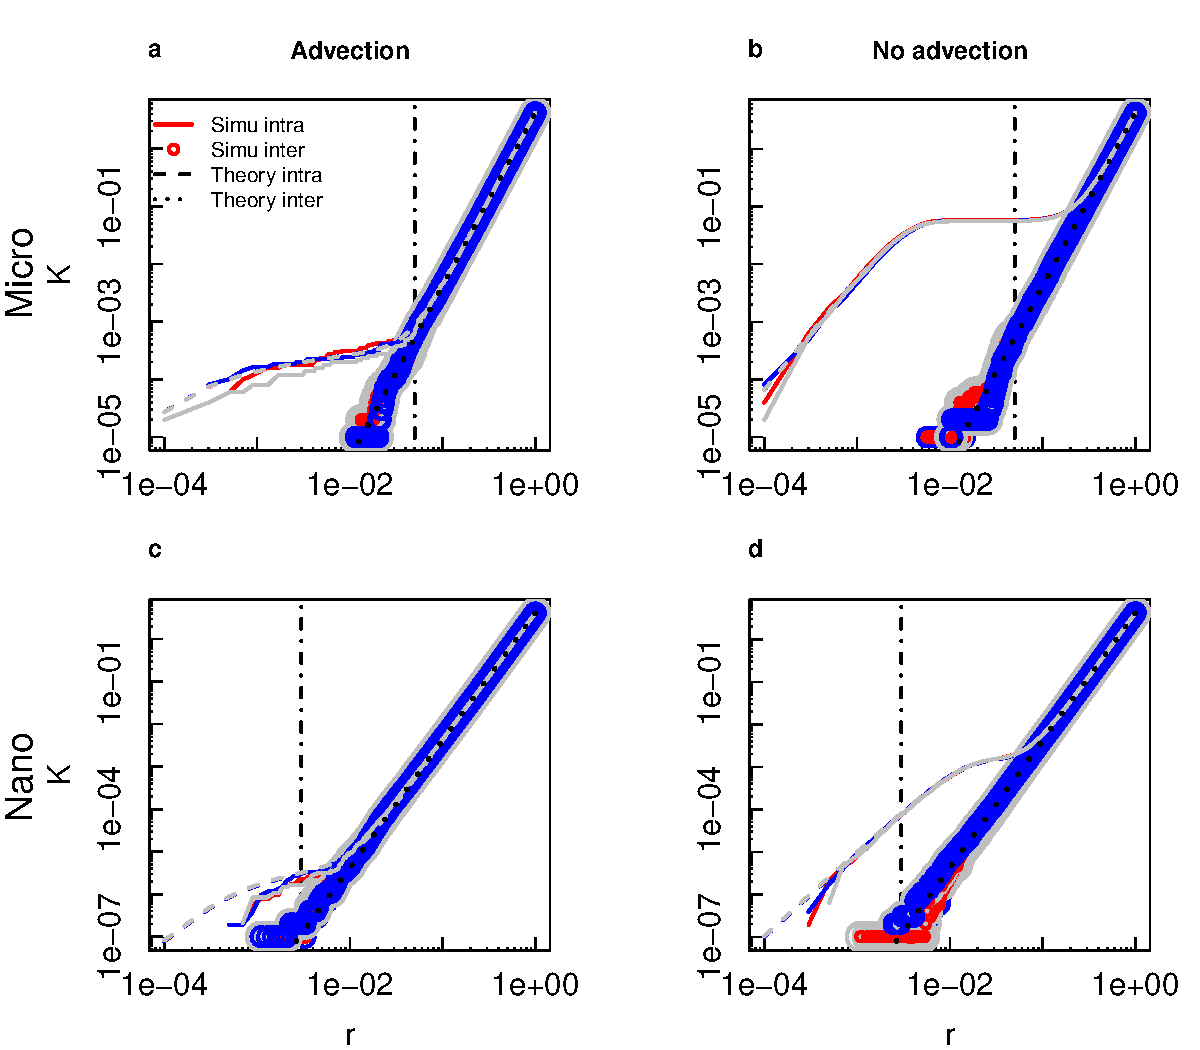
\includegraphics[width=0.99\textwidth]{../code/figure/K_micronano}
\par\end{centering}
\caption{Ripley's $K$-function as a function of distance (in cm) for microphytoplankton
(a-b) and nanophytoplankton (b-c) in a 3-species community with even
distributions after 1000 timesteps, with (a, c) and without (b, d)
advection. Each color represents a different species. The black dash-dotted
line corresponds to the threshold considered as the maximum distance
for nutrient-based competition.\label{fig:Ripley's-K-function} }
\end{figure}

Dominance indices all follow a similar pattern (Fig. \ref{fig:Dominance-3sp}
and \ref{fig:Dominance-10sp}). The dominance index is close to 1
for small distances: there is always a scale at which an organism
is surrounded almost only by conspecifics. The index then decreases
sharply to converge at large distances (close to 1 cm) to the proportion
of the focus species in the whole community, as it would for a uniform
distribution. Patterns differ at intermediate ranges of distances
between organisms.

In the presence of advection, the dominance index starts decreasing
for a distance between 5 and 10 times lower than when advection is
absent, which indicates that organisms are closer to heterospecifics
when their environment is turbulent. A quasi-uniform distribution
is also reached for smaller distances with advection than without.
Microphytoplankton species start mixing for distances larger than
for nanophytoplankton species irrespective of the hydrodynamic regime
surrounding them.

In a 3-species community with the same initial abundances, microphytoplankton
dominance indices are between 0.37 and 0.47 at the distance threshold
for potential interactions, while it is between 0.80 and 0.94 for
nanophytoplankton species when advection is present. In the absence
of turbulence, dominance indices are all above 0.98 when the distance
threshold is reached (Fig. \ref{fig:Dominance-3sp}). Microphytoplankton
organisms are therefore as likely to share their depletion volume
with conspecifics as they are with heterospecifics, but only when
turbulent advection is accounted for, whereas nanophytoplankton organisms
have almost only conspecifics around them.

\begin{figure}[H]
\begin{centering}
\includegraphics[width=0.99\textwidth]{../code/figure/dominance_diatom_nano_compare_advection}
\par\end{centering}
\caption{Dominance indices as a function of distance (in cm) for microphytoplankton
(a) and nanophytoplankton (b) in a 3-species community with even distributions
after 1000 timesteps, with (circles) and without (lines) advection.
Each color represents a different species. The black dashed line corresponds
to the threshold considered as the maximum distance for nutrient-based
competition.\label{fig:Dominance-3sp} }
\end{figure}

These differences between microphytoplankton and nanophytoplankton,
and the role of advection, are even more pronounced when considering
a 10 species-community with a skewed abundance distribution. (Fig.
\ref{fig:Dominance-10sp}). In the presence of advection, microphytoplankton
dominance indices at the distance threshold are between 0.34 (for
the most abundant species) and 0.033 (for one of the least abundant
species), while they are between 0.90 and 0.85 when advection is not
taken into account. Nanophytoplankton species, too, are more mixed:
dominance indices vary between 0.54 and 0.2 when the depletion-zone
limit is reached (with an exception of 0 for one particular species
which had no conspecific for radii below $10^{-2}$ cm) when organisms
are displaced by turbulence, while the same quantity is between 1
and 0.97 when they are only subject to diffusion.

\begin{figure}[H]
\begin{centering}
\includegraphics[width=0.99\textwidth]{../code/figure/dominance_diatom_nano_compare_advection_10sp}
\par\end{centering}
\caption{Dominance indices as a function of distance (in cm) for microphytoplankton
(a) and nanophytoplankton (b) in a 10-species community with a skewed
abundance distribution (final proportion in the community is indicated
in the legend) after 1000 timesteps, with (circles) and without (lines)
advection. Each color represents a different species. The black dashed
line corresponds to the threshold considered as the maximum distance
for nutrient-based competition.\label{fig:Dominance-10sp}}
\end{figure}

Differences in spatial distributions are not only due to organism
sizes, which determine properties of demography and turbulence, but
also to their abundances (here set through initial values). In the
presence of turbulence, the threshold distance at which dominance
falls below 95\% is smaller for more abundant species (Fig. \ref{fig:Carac_10sp}
a-b). Abundant species tend to be present nearly everywhere when they
are mixed in the environment. Therefore, they are also more likely
to be close to a heterospecific, but still have more conspecifics
close to them than the less abundant species ($D_{\text{threshold}}$
increases with abundance, Fig. \ref{fig:Carac_10sp} c-d). However,
this increase is less marked for nanophytoplankton than for microphytoplankton
(Fig. \ref{fig:Carac_10sp} c-d). When turbulence is absent, the relationships
with abundance are unclear, possibly affected by sampling effects,
and we refrain from interpreting them.

\begin{figure}[H]
\begin{centering}
\includegraphics[width=0.8\textwidth]{../code/figure/carac_10species}
\par\end{centering}
\caption{Minimum distances (in cm) between points for dominance to drop below
95\% (a and b) and dominance at a distance corresponding to the threshold
for competition (c and d) as a function of abundances (note the logarithmic
scale on the x-axis) for microphytoplankton and nanophytoplankton.
We consider cases with and without advection in a 10-species community
with a skewed abundance distribution. \label{fig:Carac_10sp}}
\end{figure}


\section*{Discussion}

We designed a stochastic, three-dimension, individual-based model
of the spatial distribution of multiple species in a viscous and turbulent
flow. We conducted both mathematical analyses and numerical simulations
to quantify spatial correlations in organism distributions. We focused
on the pair correlation function and Ripley's $K$-function, for which
numerical and theoretical analyses showed a good agreement, and extracted
a more ecologically-oriented metric from them, \textit{i.e.} the dominance
index. This statistic is the \textit{local} average ratio of conspecifics,
i.e., the number of organisms of the focal species in the neighbourhood
of an individual of the same species, divided by the total number
of organisms in that neighborhood. Intraspecific clustering corresponds
to a dominance index close to 1, which decreases when interspecific
mixing increases. The choice of this index was motivated by two reasons:
it is at its core a proportion of a focus species in a certain volume,
i.e. a scale-dependent, localized metric bounded between 0 and 1 as
opposed to other statistics whose values are less directly interpreted,
and is easy to relate to coexistence theory as it describes the environment
of an organism in terms of heterospecifics and conspecifics, which
can, under certain hypotheses that we discuss below, be related to
interspecific and intraspecific interactions. Comparing the distributions
of organisms of different sizes and demography, we showed that the
presence and intensity (Section S8 of the SI) of turbulence always
increased mixing, and that the species composition around an organism
depended on its size, which mechanically determines its hydrodynamics
properties (diffusivity), and is linked with its ecological characteristics
(growth rate and density). Microphytoplankters (20 to 200 \textmu
m), larger cells with lower diffusivity, growth rate and abundance,
were on average further away from other cells, due to their lower
concentrations (Section S6 of the SI), than nanophytoplankters (2
to 20 \textmu m). However, they were surrounded by more heterospecifics
than conspecifics within a volume of potential interactions, whose
radius is defined as the maximum distance for which nutrient depletion
volumes of two different individuals may overlap. If we consider that
interactions between species (not modelled here), could occur with
equal probability at all distances within the volume of potential
interactions, we would conclude that microphytoplankters are more
likely to interact with individuals from other species than with individuals
of their own species. However,this affirmation is conditional upon
interactions at 10 cell diameters from an individual being equally
likely than at 1 diameter from an individual. If we keep in mind that
interactions are more likely or stronger at very short distances,
microphytoplankters may still experience more frequent effects of
conspecifics than heterospecifics.

To see this, let us first focus on the smallest distances between
organisms. The nearest neighbour of an organism was always an organism
of the same species, and the minimum distance between conspecifics
was always lower than expected for a uniform distribution (Section
S6). The dominance index remained close to 1 for distances below $10^{-2}$
cm or $10^{-3}$ cm for microphytoplankton and nanophytoplankton respectively.
There was therefore always \emph{some} intraspecific aggregation,
i.e. conspecifics were always closer than heterospecifics at the lowest
distances. This is due to the prevalence of demographic processes
at individual scales, because an individual acts as a source point
for other organisms of the same species, and hydrodynamic processes
do not separate conspecifics fast enough to prevent aggregation. If
we consider that interaction strengths are a smoothly decaying function
of distance, a common assumption in spatial coexistence models \citep[e.g., ][]{bolker_spatial_1999,law_population_2003},
this implies that population-level intraspecific interactions could
be stronger than interspecific interactions due to intraspecific micro-scale
aggregation. However, the mechanisms of competition at this scale
are poorly known, likely relying on multiple types of resources with
different distributions in the environment, effects on the cell, uptakes,
etc. Rather than weighting much more heavily the potential interactions
with the closest neighbour(s) through an interaction kernel, we therefore
chose conservatively to define a maximum distance for two organisms
to possibly affect the concentrations of elements in the environment
of each other. We consider that, at all distances below this threshold,
interaction could happen between organisms. We continue the discussion
with that simplification in mind, and explicitely mention when it
is relaxed.

Dominances began to decrease at distances above $10^{-3}$ cm, still
below the maximum distance for interactions. At this distance and
above, the balance between heterospecifics and conspecifics was much
more sensitive to different phytoplankton's demographics and hydrodynamic
traits. The species composition of an organism's neighbourhood depended
on its size: nanophytoplankton organisms mainly shared their volume
of potential interactions with conspecifics (the dominance index remained
close to 1, even near the distance threshold, i.e. the maximum distance
for nutrient depletion volume overlap) while microphytoplankton organisms
could affect both conspecifics and heterospecifics (the dominance
index was often below 50\% at the distance threshold, i.e. a particle's
depletion zone probably overlapped with more heterospecifics' than
conspecifics'). Microphytoplankters were therefore more likely to
share their depletion volume with heterospecifics than nanophytoplankters.
The rate of production of new microphytoplankton conspecifics was
not sufficient to compensate for the separation velocity due to turbulence
and diffusivity, even though the diffusion range of microphytoplankters
was smaller than that of nanophytoplankters. There may therefore be
different mechanisms at play at the community level for microphytoplankton
and nanophytoplankton. For nanophytoplankton, the spatial structure
likely leads to more interactions between conspecifics than between
heterospecifics. The distribution of microphytoplankton species, on
the contrary, encourages more interactions between heterospecifics.
If we consider that local interaction strengths are equal within the
volume of potential interactions, scaling to the population level,
we would likely observe stronger intra- over interspecific interactions
for nanophytoplankton (a key factor in coexistence theory, \citealp{barabas_self-regulation_2017})
but not necessarily so for microphytoplankton.

All of the above discussion is based on a microphytoplankter's neighbourhood
as defined by nutrient depletion volumes. To simplify the computation,
we used maximum volumes of potential interaction, corresponding to
a diffusive-only flow of nutrient particles. But when fluid turbulence
increases, nutrient uptake increases due to that turbulence, and the
size of the depletion zone decreases \citep{karp-boss_nutrient_1996}.
The proportion of change in the depletion volume increases with the
size of organism: a 10 \textmu m-diameter organism might not experience
any change, while the uptake of a 100 \textmu m-diameter organism
would increase by at least 50\% \citep{karp-boss_nutrient_1996}.
Therefore the volume of potential interactions shrinks in the presence
of turbulence for microphytoplankton, but not necessarily for nanophytoplankton.
This is one additional reason why microphytoplankers might still be
surrounded by conspecifics at ecologically meaningful distances and
interacting more frequently with them.

Up to now, we have only focused on the dominance index, a localized
proportion of conspecifics. However, interactions also depend on the
absolute densities of individuals. Mechanically, when density decreases,
the distances between neighbours increase, which explains that the
distances between the low-abundance microphytoplankters tended to
be greater than distances between the more abundant nanophytoplankters
(Section S6 of the SI). Explicit mathematical models using pair densities
to express interaction rates \citep[e.g.][]{law_population_2003,plank_spatial_2015}
may be able to incorporate those effects; however, as we highlight
below, the timescales and spatial correlations that develop in such
models may not necessarily represent faithfully phytoplankton community
dynamics. 

Contrary to other similar models \citep[e.g.,][]{birch_master_2006,bouderbala_3d_2018},
we did not consider explicit effects of local density on survival
and fertility rates. Outside of simply maintaining analytical tractability,
we had another, more biological reason to do so: we cannot be sure
that these local density-dependencies make sense in our phytoplankton
context. To understand why, consider that even if a species abundance
is locally tripled, competition might not directly ensue at the time
scales covered by our model, if nutrient depletion has not had time
to set in yet. We would need lagged local density-dependencies, which
are to our knowledge not leading to tractable spatial branching or
dynamic point processes. We could, of course, directly model nutrients,
perhaps as resource ``points'' with a dynamics of their own \citep{murrell_local_2005,north_interactions_2007},
which in turn change the reproduction or death rate of individuals.
If the resource points risk being depleted, this entails a negative
spatial correlation between organisms and their resources \citep{murrell_local_2005}.
And that is where such models might be inadequate. The phycosphere,
a micro-environment at the periphery of a phytoplankton organism where
communities of bacteria interact \citep{seymour_zooming_2017}, can
also impact phytoplankton fitness, both positively (cross-feeding)
and negatively (algicidal activities of bacteria). This can sometimes
lead to an accumulation of key resources close to the phytoplankter.
This will lead to positive spatial correlations between consumers
and their resources, and we currently do not have theoretical models
to represent this (short of modelling precisely these bacteria). 

Our model should be viewed as a first model of spatial distributions
of multiple phytoplankton species in a realistic, three-dimensional
environment at the microscale, describing only basic hydrodynamic
and demographic processes. Using this model, we were able to guesstimate
the differences in potential intra vs interspecific interactions between
species, emerging at the population level through spatial distributions
\citep{detto_stabilization_2016}. It is worthwhile to keep in mind
that there are numerous remaining features of phytoplankton physiology
and life histories which we do not cover here, but may affect their
spatial distributions. Many phytoplankters are able to move actively
in three-dimensions, which can favour cluster formation \citep{breier_emergence_2018}.
Even those who are believed to move passively actually often move
along the vertical dimension by regulating their buoyancy \citep{reynolds2006ecology},
and can at times aggregate to form pairs \citep{font-munoz_collective_2019}. Finally, a
part of spatial structure is explained by the partially colonial nature
of microphytoplankton \citep{kiorboe_coagulation_1990}. This clearly
calls for viewing our model as a null model to which more complex
mechanistic models and their spatial outputs can be compared.

\subsubsection*{Declaration of Competing Interest}

The authors declare that they have no known competing financial interests
or personal relationships that could have appeared to influence the
work reported in this paper.

\subsubsection*{Author contribution statement}

\subsubsection*{Acknowledgments}

FB and CP were supported by the grant ANR-20-CE45-0004. CP was supported
by a PhD grant from the French Ministry of Research.

\section*{Appendices}

\renewcommand\thesection{A\arabic{section}}
\setcounter{section}{0}
\renewcommand\thefigure{A\arabic{figure}}
\setcounter{figure}{0}
\renewcommand\thetable{A\arabic{table}}

\subsection*{Derivation of the spatial characteristics of the Brownian Bug Model}

We show here how to compute the monospecific pair correlation function
and Ripley's $K$-function of the Brownian Bug Model. Formula for
standard processes are given in the Supplementary Information, for
readers who want to familiarize with simpler models. 

\subsubsection*{Proof of eq. \ref{eq:pcf_intraspecific}}

In three dimensions, when the birth rate $\lambda$ is the same as
the mortality rate $\mu$, the pair density $G(r)$  is a solution
of eq. \ref{eq:Young3D-1} (see \citealp{young_reproductive_2001}
and \citealp{picoche_rescience_2022} for a detailed derivation).

\begin{equation}
\frac{\partial G}{\partial t}=\frac{2D}{r^{2}}\frac{\partial}{\partial r}\left(r^{2}\frac{\partial G}{\partial r}\right)+\frac{\gamma}{r^{2}}\frac{\partial}{\partial r}\left(r^{4}\frac{\partial G}{\partial r}\right)+2\lambda C\delta(\boldsymbol{r})\label{eq:Young3D-1}
\end{equation}


\paragraph{With advection}

In the presence of advection ($\gamma\neq0$), a steady-state solution
can be found. 

\begin{onehalfspace}
\noindent 
\begin{align}
 & \,0 & = & \frac{2D}{r^{2}}\frac{\partial}{\partial r}\left(r^{2}\frac{\partial G}{\partial r}\right)+\frac{\gamma}{r^{2}}\frac{\partial}{\partial r}\left(r^{4}\frac{\partial G}{\partial r}\right)+2\lambda C\delta(\boldsymbol{r})\nonumber \\
\Leftrightarrow & \,0 & = & 4\pi r^{2}\left(\frac{2D}{r^{2}}\frac{\partial}{\partial r}\left(r^{2}\frac{\partial G}{\partial r}\right)+\frac{\gamma}{r^{2}}\frac{\partial}{\partial r}\left(r^{4}\frac{\partial G}{\partial r}\right)+2\lambda C\delta(\boldsymbol{r})\right)\nonumber \\
\Leftrightarrow & \,0 & = & 4\pi\left(2D\frac{\partial}{\partial r}\left(r^{2}\frac{\partial G}{\partial r}\right)+\gamma\frac{\partial}{\partial r}\left(r^{4}\frac{\partial G}{\partial r}\right)\right)+4\pi r^{2}2\lambda C\delta(\boldsymbol{r})\label{eq:steady_state}
\end{align}

\end{onehalfspace}

We can then integrate Eq. (\ref{eq:Young3D-1}) over a small sphere
centered on a particle, with radius $\rho$. Let us first note that

\begin{onehalfspace}
\noindent 
\begin{eqnarray}
\int_{\mathbb{R}^{3}}\delta(\boldsymbol{r})d^{3}\boldsymbol{r} & = & 1\nonumber \\
\Leftrightarrow\int_{0}^{2\pi}\int_{0}^{\pi}\int_{0}^{\rho}\delta(\boldsymbol{r}')r'^{2}\sin(\phi) & dr' & d\phi d\theta=1\nonumber \\
\Leftrightarrow4\pi\int_{0}^{\rho}\delta(\boldsymbol{r}')r'^{2}dr' & = & 1\label{eq:delta_integration}
\end{eqnarray}

\end{onehalfspace}

Using Eq. (\ref{eq:steady_state}) and (\ref{eq:delta_integration}), 

\begin{onehalfspace}
\noindent 
\begin{align}
 & 0 & = & 4\pi\left(2Dr^{2}\frac{\partial G}{\partial r}+\gamma r^{4}\frac{\partial G}{\partial r}\right)+2\lambda C\nonumber \\
\Leftrightarrow & \frac{\partial G}{\partial r} & = & -\frac{1}{4\pi}\frac{2\lambda C}{2Dr^{2}+\gamma r^{4}}\label{eq:deriv_G_r}
\end{align}

\end{onehalfspace}

We can integrate between $\rho$ and $\infty$, knowing that $G(\infty)=C^{2}.$

\begin{onehalfspace}
\noindent 
\begin{align}
 & C^{2}-G(\rho) & = & -\frac{2\lambda C}{4\pi}{\displaystyle \int_{\rho}^{\infty}}\frac{1}{2Dr^{2}+\gamma r^{4}}dr\label{eq:deriv_G_r_int1}
\end{align}

\end{onehalfspace}

We first compute the primitive $A=\int\frac{1}{2Dr^{2}+\gamma r^{4}}dr$. 

\begin{equation}
\begin{array}{ccc}
A & = & \int\frac{1}{r^{2}\left(2D+\gamma r^{2}\right)}dr\\
 & = & \int\frac{1}{2Dr^{2}}-\frac{\gamma}{2D\left(2D+\gamma r^{2}\right)}dr\\
 & = & \frac{1}{2D}\int\frac{1}{r^{2}}dr-\frac{\gamma}{2D}\int\frac{1}{2D+\gamma r^{2}}dr\\
 & = & -\frac{1}{2Dr}-\frac{\gamma}{2D}\int\frac{1}{2D\left(1+\left(\sqrt{\frac{\gamma}{2D}}r\right)^{2}\right)}
\end{array}
\end{equation}

With a change of variable $u=\sqrt{\frac{\gamma}{2D}}r$, using $\int\frac{1}{1+u^{2}}=\arctan(u)$,
we have:

\begin{equation}
A=-\frac{1}{2Dr}-\frac{\sqrt{\gamma}\arctan\left(\frac{\sqrt{\gamma}r}{\sqrt{2D}}\right)}{2\sqrt{2}D\sqrt{D}}+K
\end{equation}

where $K$ is a constant.

We can know compute $B=[A]_{\rho}^{\infty}.$ 

\begin{equation}
B=-\frac{\sqrt{\gamma}\pi}{4\sqrt{2}D\sqrt{D}}+\frac{1}{2D\rho}+\frac{\sqrt{\gamma}\arctan\left(\frac{\sqrt{\gamma}\rho}{\sqrt{2D}}\right)}{2\sqrt{2}D\sqrt{D}}
\end{equation}

This leads to:

\begin{equation}
\begin{array}{ccc}
G(\rho) & = & C^{2}+\frac{2\lambda C}{4\pi}B\\
 & = & C^{2}+\frac{\lambda C}{2\pi}\left[\frac{1}{2D\rho}+\frac{\sqrt{\gamma}\arctan\left(\frac{\sqrt{\gamma}\rho}{\sqrt{2D}}\right)}{2\sqrt{2}D\sqrt{D}}-\frac{\sqrt{\gamma}\pi}{4\sqrt{2}D\sqrt{D}}\right].
\end{array}
\end{equation}

Finally, the pair correlation function $g=G/C^{2}$ is defined as

\begin{equation}
g(\rho)=\frac{\lambda}{4\pi CD}\left(\frac{\sqrt{\gamma}\arctan\left(\frac{\sqrt{\gamma}\rho}{\sqrt{2D}}\right)}{\sqrt{2D}}+\frac{1}{\rho}-\frac{\pi\sqrt{\gamma}}{2\sqrt{2D}}\right)+1.\label{eq:pcf_adv_bbm}
\end{equation}


\paragraph{Without advection}

When $U=0$, $\gamma=0$ and there is no steady solution. We can get
back to Eq. (\ref{eq:Young3D-1}). 

\begin{equation}
\frac{\partial G}{\partial t}=\frac{2D}{r^{2}}\frac{\partial}{\partial r}\left(r^{2}\frac{\partial G}{\partial r}\right)+2\lambda C\delta(\boldsymbol{r})
\end{equation}

Assuming an isotropic environment, this means

\begin{equation}
\frac{\partial G}{\partial t}-2D\Delta G=2\lambda C\delta(\boldsymbol{r})
\end{equation}

where $\Delta=\nabla^{2}$ is the Laplacian operator. 

We therefore have 

\begin{equation}
\mathcal{L}G(\boldsymbol{r},t)=2\lambda C\delta(\boldsymbol{r})
\end{equation}

where $\mathcal{L}$ is the linear differential operator $\partial_{t}-2D\Delta$. 

Using the Green's function theory, we know that $G(y)=\int H(y,s)2\lambda C\delta(s)ds$
where $H(y,s)=H(y-s)$ is the Green kernel (heat kernel).

\begin{align*}
 & G(\boldsymbol{r},t) & = & 2\lambda C\int_{\mathbb{R}^{3}}\int_{0}^{t}H(\boldsymbol{r}-\boldsymbol{r'},t')\delta(\boldsymbol{r'})dr'dt'\\
\Leftrightarrow &  & = & 2\lambda C\int_{0}^{t}H(\boldsymbol{r},t')dt'
\end{align*}

A solution for the Green's function using $\mathcal{L}=\partial_{t}-2D\Delta$
in 3 dimensions is $H(r,t)=\left(\frac{1}{4\pi2Dt}\right)^{3/2}\exp(\frac{-r^{2}}{4\times2Dt})$.

$G(r,t)$ can then be computed:

.
\begin{equation}
G(r,t)=2\lambda C\left(\frac{-\erf\left(\frac{r}{\sqrt{8tD}}\right)}{8\pi Dr}+K\right)\label{eq:G_r_t}
\end{equation}

where $\erf$ is the error function. Using $G(r,0)=C^{2}$ and $\lim_{x\rightarrow+\infty}\erf(x)=1$
in Eq. (\ref{eq:G_r_t}), 

\begin{equation}
\begin{array}{ccc}
C^{2} & = & 2\lambda C\left(\frac{1}{8\pi Dr}+K\right)\\
\Leftrightarrow\frac{C}{2\lambda}- & \frac{1}{8\pi Dr}= & K
\end{array}
\end{equation}

We can finally compute $G(r,t)$:

\begin{equation}
\begin{array}{ccc}
G(r,t) & = & 2\lambda C\left(-\frac{\erf\left(\frac{r}{\sqrt{8tD}}\right)}{8\pi Dr}+\frac{C}{2\lambda}+\frac{1}{8D\pi r}\right)\\
 & = & \frac{\lambda C}{4\pi Dr}\left\{ 1-\erf\left(\frac{r}{\sqrt{8Dt}}\right)\right\} +C^{2}\\
\Leftrightarrow g(r,t) & = & \frac{\lambda}{4D\pi rC}\left\{ 1-\erf\left(\frac{r}{\sqrt{8Dt}}\right)\right\} +1.
\end{array}\label{eq:pcf_noadv_bbm}
\end{equation}


\subsubsection*{Proof of eq. \ref{eq:K_intraspecific}}

We can integrate the pcf formula to compute Ripley's $K$-function,
as $g(r)=\frac{K'(r)}{4\pi r^{2}}$. 

\paragraph{With advection}

From eq. \ref{eq:pcf_adv_bbm}, 

\begin{equation}
\begin{array}{ccc}
K(\rho) & = & 4\pi\int_{0}^{\rho}r^{2}+\frac{\lambda}{2\pi C}\left[\frac{r}{2D}+\frac{\sqrt{\gamma}r^{2}\arctan\left(\frac{\sqrt{\gamma}r}{\sqrt{2D}}\right)}{2\sqrt{2}D\sqrt{D}}-\frac{\sqrt{\gamma}\pi r^{2}}{4\sqrt{2}D\sqrt{D}}\right]dr.\end{array}\label{eq:start-K}
\end{equation}

We define $A=\int_{0}^{\rho}r^{2}dr$ , $B=\int_{0}^{\rho}\frac{r}{2D}dr$,
$C=\int_{0}^{\rho}r^{2}\arctan\left(\frac{\sqrt{\gamma}r}{\sqrt{2D}}\right)dr$
and $E=\int_{0}^{\rho}\frac{\sqrt{\gamma}\pi r^{2}}{4\sqrt{2}D\sqrt{D}}dr$. 

\begin{equation}
\begin{array}{cc}
A= & \frac{1}{3}\rho^{3}\\
B= & \frac{\rho^{2}}{4D}\\
E= & \frac{\sqrt{\gamma}\pi\rho^{3}}{12\sqrt{2}D\sqrt{D}}
\end{array}
\end{equation}

We can also compute $C=\int_{0}^{\rho}r^{2}\arctan\left(\frac{\sqrt{\gamma}r}{\sqrt{2D}}\right)dr$.
We can first change variable, with $u=\frac{r}{\sqrt{2D}},$$dr=\sqrt{2D}du$.

\begin{equation}
\begin{array}{ccc}
C & = & \int_{0}^{\rho/\sqrt{2D}}(\sqrt{2D}u)^{2}\arctan(\sqrt{\gamma}u)\sqrt{2D}du\\
 & = & (2D)^{3/2}\int_{0}^{\rho/\sqrt{2D}}u^{2}\arctan(\sqrt{\gamma}u)du
\end{array}
\end{equation}

We can integrate by parts, with $f=\arctan(\sqrt{\gamma}u)$ and $g'=u^{2}$.

\begin{equation}
\begin{array}{ccc}
C & = & (2D)^{3/2}\left(\frac{\rho^{3}}{3(2D)^{3/2}}\arctan(\sqrt{\frac{\gamma}{2D}}\rho)-\int_{0}^{\rho/\sqrt{2D}}\frac{\sqrt{\gamma}u^{3}}{3(\gamma u^{2}+1)}du\right)\\
 & = & (2D)^{3/2}\left(\frac{\rho^{3}}{3(2D)^{3/2}}\arctan(\sqrt{\frac{\gamma}{2D}}\rho)-\frac{\sqrt{\gamma}}{3}\int_{0}^{\rho/\sqrt{2D}}\frac{u^{3}}{(\gamma u^{2}+1)}du\right)
\end{array}
\end{equation}

We can substitute $v=\gamma u^{2}+1,$$du=\frac{1}{2\gamma u}dv$.

\begin{equation}
\begin{array}{ccc}
\int_{0}^{\rho/\sqrt{2D}}\frac{u^{3}}{(\gamma u^{2}+1)}du & = & \frac{1}{2\gamma^{2}}\int_{1}^{\gamma\rho^{2}/2D+1}\frac{v-1}{v}dv\\
 & = & \frac{1}{2\gamma^{2}}\int_{1}^{\gamma\rho^{2}/2D+1}1-\frac{1}{v}dv\\
 & = & \frac{1}{2\gamma^{2}}(\gamma\frac{\rho^{2}}{2D}-\log(\gamma\frac{\rho^{2}}{2D}+1))
\end{array}
\end{equation}

Going back to C, we obtain:

\begin{equation}
\begin{array}{ccc}
C & = & \frac{\rho^{3}\arctan(\sqrt{\frac{\gamma}{2D}}\rho)}{3}-\left(2D\right)^{3/2}\frac{\sqrt{\gamma}}{3}\frac{1}{2\gamma^{2}}\left(\frac{\gamma}{2D}\rho^{2}-\log(\gamma\frac{\rho^{2}}{2D}+1)\right)\\
 & = & \frac{\rho^{3}\arctan(\sqrt{\frac{\gamma}{2D}}\rho)}{3}-\frac{\sqrt{2D}}{6\sqrt{\gamma}}\rho^{2}+\frac{\sqrt{2}D^{3/2}}{3\gamma^{3/2}}\log(\gamma\frac{\rho^{2}}{2D}+1).
\end{array}
\end{equation}

Combining all equations:

\begin{equation}
\begin{array}{ccc}
K(\rho) & = & \frac{4}{3}\pi\rho^{3}+\frac{2\lambda}{C}\left(\frac{\rho^{2}}{4D}+\frac{\sqrt{\gamma}\rho^{3}\arctan(\sqrt{\frac{\gamma}{2D}}\rho)}{6\sqrt{2}D^{3/2}}-\frac{\rho^{2}}{12D}+\frac{\log\left(\gamma\frac{\rho^{2}}{2D}+1\right)}{6\gamma}-\frac{\sqrt{\gamma}\pi\rho^{3}}{12\sqrt{2}D\sqrt{D}}\right)\\
 & = & \frac{4}{3}\pi\rho^{3}+\frac{2\lambda}{C}\left(\frac{\rho^{2}}{6D}+\frac{\sqrt{\gamma}\rho^{3}\arctan(\sqrt{\frac{\gamma}{2D}}\rho)}{6\sqrt{2}D^{3/2}}+\frac{\log\left(\gamma\frac{\rho^{2}}{2D}+1\right)}{6\gamma}-\frac{\sqrt{\gamma}\pi\rho^{3}}{12\sqrt{2}D\sqrt{D}}\right).
\end{array}
\end{equation}


\paragraph{Without advection}

From eq. \ref{eq:pcf_noadv_bbm},

\paragraph{
\begin{equation}
\protect\begin{array}{ccc}
K(\rho) & = & \frac{\lambda}{DC}\int_{0}^{\rho}r\left\{ 1-\erf\left(\frac{r}{\sqrt{8Dt}}\right)\right\} +4\pi r^{2}dr\protect\\
 & = & \frac{\lambda}{CD}\left(\frac{\rho^{2}}{2}-\int_{0}^{\rho}r\times\erf\left(\frac{r}{\sqrt{8Dt}}\right)dr\right)+\frac{4}{3}\pi\rho^{3}
\protect\end{array}
\end{equation}
}

We first compute the primitive for $\int_{0}^{\rho}r\times\erf\left(\frac{r}{\sqrt{8Dt}}\right)dr$.
We define $u=\frac{r}{\sqrt{8Dt}}$, $dr=\sqrt{8Dt}du$.

\begin{equation}
\begin{array}{ccc}
\int_{0}^{\rho}r\times\erf\left(\frac{r}{\sqrt{8Dt}}\right)dr & = & 8Dt\int_{0}^{\rho/\sqrt{8Dt}}u\times\erf\left(u\right)du\end{array}
\end{equation}

We can integrate by parts, with $f=\erf(u)$ and $g'=u$.

\begin{equation}
\begin{array}{ccc}
8Dt\int_{0}^{\rho/\sqrt{8Dt}}u\times\erf\left(u\right)du & = & 8Dt\left(\frac{\rho^{2}}{2}\frac{1}{8Dt}\erf(\frac{\rho}{\sqrt{8Dt}})-\frac{1}{\sqrt{\pi}}\int_{0}^{\rho/\sqrt{8Dt}}u^{2}e^{-u^{2}}du\right)\end{array}\label{eq:parts}
\end{equation}

We integrate by parts again, this time with $f=u$ and $g'=ue^{-u^{2}}$,
which leads to 

\begin{equation}
\int u^{2}e^{-u^{2}}du=-\frac{ue^{-u^{2}}}{2}+\frac{1}{2}\int e^{-u^{2}}du=-\frac{ue^{-u^{2}}}{2}+\frac{\sqrt{\pi}\erf(u)}{4}\label{eq:integrate_parts}
\end{equation}

If we use eq. \ref{eq:integrate_parts} in eq. \ref{eq:parts}:

\begin{equation}
\begin{array}{ccc}
8Dt\int_{0}^{\rho/\sqrt{8Dt}}u\times\erf\left(u\right)du & = & 8Dt\left(\frac{\rho^{2}}{2}\frac{1}{8Dt}\erf(\frac{\rho}{\sqrt{8Dt}})-\frac{\erf(\frac{\rho}{\sqrt{8Dt}})}{4}+\frac{1}{2\sqrt{\pi}}\frac{\rho}{\sqrt{8Dt}}e^{-\rho^{2}/8Dt}\right)\\
\Leftrightarrow\int_{0}^{\rho}r\times\erf\left(\frac{r}{\sqrt{8Dt}}\right)dr & = & \frac{1}{2}\erf(\frac{\rho}{\sqrt{8Dt}})(\rho^{2}-4Dt)+\frac{\sqrt{2Dt}}{\sqrt{\pi}}\rho e^{-\rho^{2}/8Dt}
\end{array}
\end{equation}

We can now compute $K(\rho)$:

\begin{equation}
\begin{array}{ccc}
K(\rho) & = & \frac{\lambda}{CD}\left(\frac{\rho^{2}}{2}-\frac{1}{2}\erf(\frac{\rho}{\sqrt{8Dt}})(\rho^{2}-4Dt)-\frac{\sqrt{2Dt}\rho}{\sqrt{\pi}}e^{-\rho^{2}/8Dt}\right)+\frac{4}{3}\pi\rho^{3}.\end{array}\label{eq:end_K}
\end{equation}

\bibliographystyle{ecol_let}
\bibliography{bibliography}

\end{document}
